%!TEX root=./main.tex
\section{Simulations}

Our experiments apply the feedback alignment algorithm to two-layer networks, using a range of networks with different widths and activations. The numerical results suggest that regularization is essential in achieving alignment, in both regression and classification tasks, for linear and nonlinear models. We implement the feedback alignment procedure in PyTorch as an extension of the autograd module for backpropagation, and the training is done on V100 GPUs from internal clusters.

\paragraph{Feedback alignment on synthetic data.}

We first train two-layer networks on synthetic data, where each network $f$ shares the architecture shown in \eqref{eqn:nonlinear-network} and the data are generated by another network $f_0$ that has the same architecture but with random Gaussian weights. We present the experiments for both linear and nonlinear networks, where the activation functions are chosen to be Rectified Linear Unit (ReLU) and Hyperbolic Tangent (Tanh) for nonlinear case. We set training sample sample size to $n=50$ and the input dimension $d=150$, but vary the hidden layer width $p = 100\times 2^k$ with $k\in[7]$. During training, we take step size $\eta = 10^{-4}$ for linear networks and $\eta = 10^{-3},10^{-2}$ for ReLU and Tanh networks, respectively.


\begin{figure}[ht]
\centering
\begin{subfigure}[b]{.33\textwidth}
  \centering
  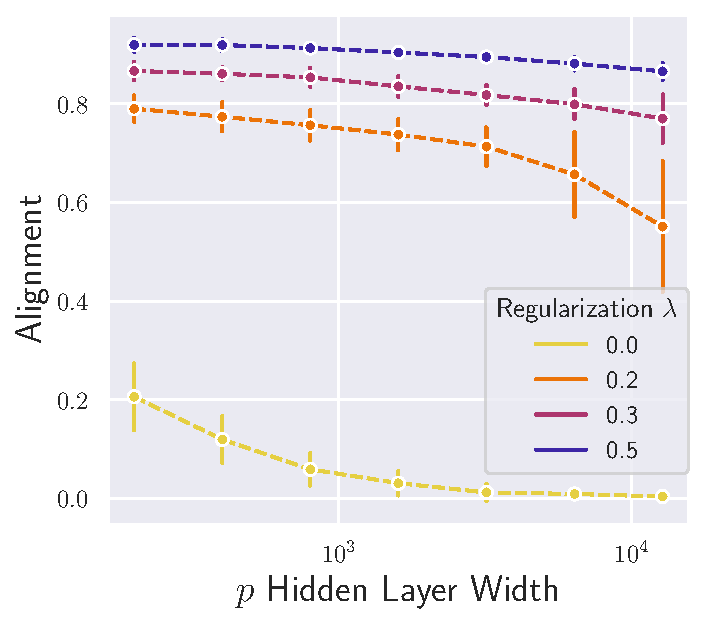
\includegraphics[width=\linewidth]{figures/df_lr_non_autograd_l2_v6.pdf}
  \caption{Alignment on linear network.}
  \label{fig:align_lr_non_autograd_l2}
\end{subfigure}\hfill
\begin{subfigure}[b]{.33\textwidth}
  \centering
  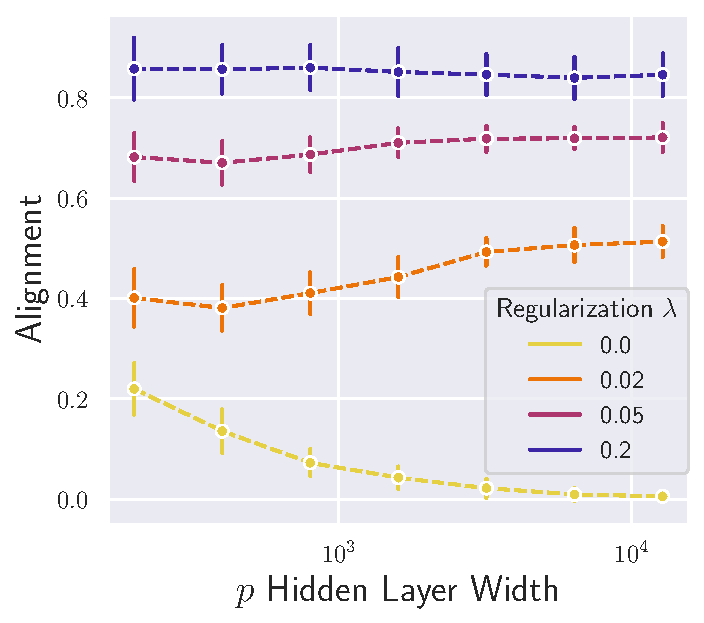
\includegraphics[width=\linewidth]{figures/df_nn_relu_autograd_l2_v6.pdf}
  \caption{Alignment on ReLU network.}
  \label{fig:align_nn_relu_autograd_l2}
\end{subfigure}\hfill
\begin{subfigure}[b]{.33\textwidth}
  \centering
  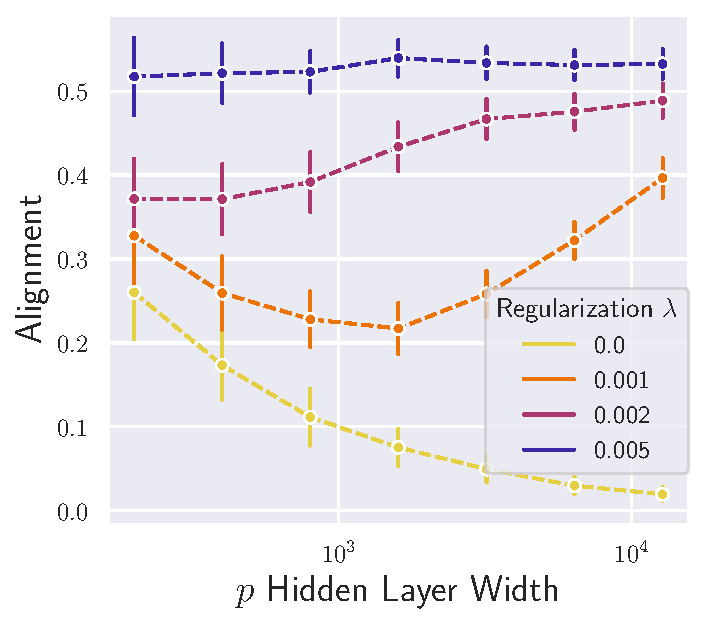
\includegraphics[width=\linewidth]{figures/df_nn_tanh_autograd_l2_v6.pdf}
  \caption{Alignment on Tanh network.}
  \label{fig:align_nn_tanh_autograd_l2}
\end{subfigure}
\medskip
\begin{subfigure}[b]{.33\textwidth}
  \centering
  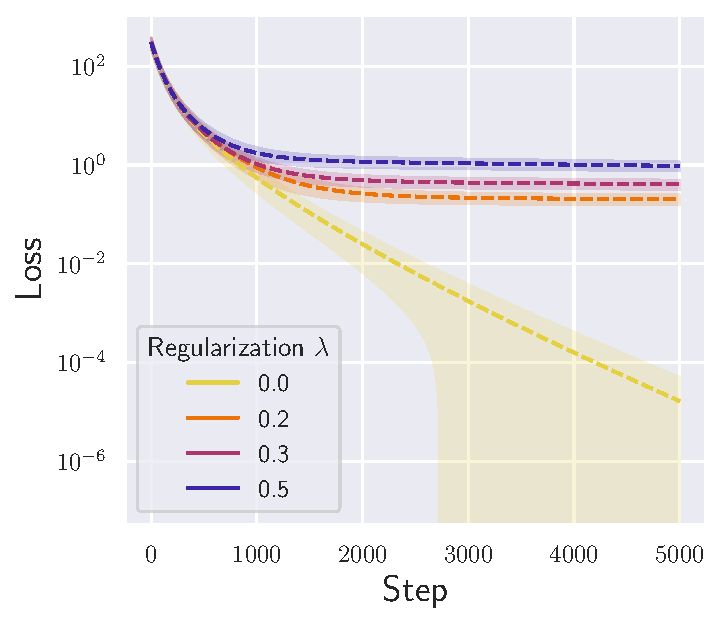
\includegraphics[width=\linewidth]{figures/loss_lr_non_autograd_l2_v1.pdf}
  \caption{Loss on linear network.}
  \label{fig:loss_lr_non_autograd_l2}
\end{subfigure}\hfill
\begin{subfigure}[b]{.33\textwidth}
  \centering
  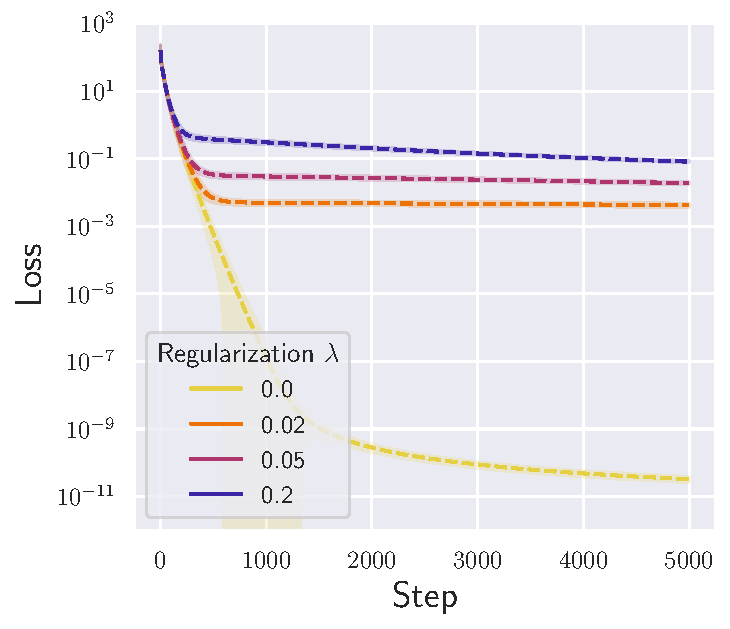
\includegraphics[width=\linewidth]{figures/loss_nn_relu_autograd_l2_v1.pdf}
  \caption{Loss on ReLU network.}
  \label{fig:loss_nn_relu_autograd_l2}
\end{subfigure}\hfill
\begin{subfigure}[b]{.33\textwidth}
  \centering
  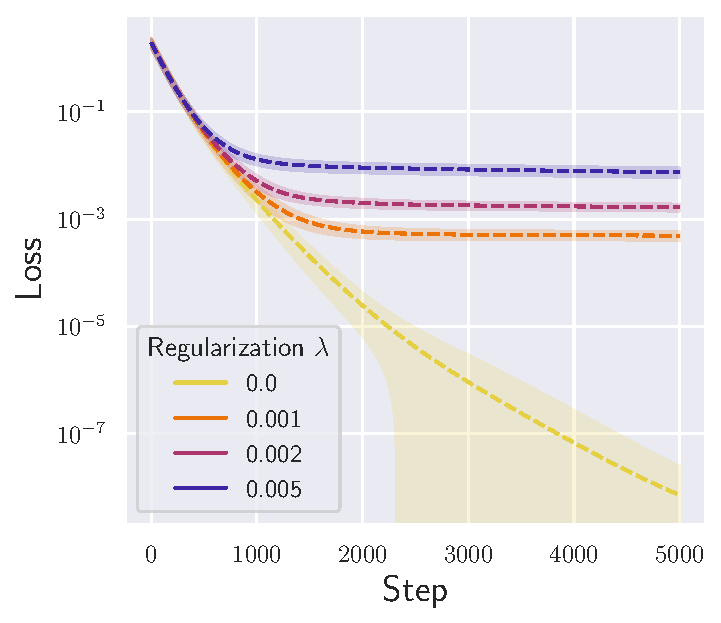
\includegraphics[width=\linewidth]{figures/loss_nn_tanh_autograd_l2_v1.pdf}
  \caption{Loss on Tanh network.}
  \label{fig:loss_nn_tanh_autograd_l2}
\end{subfigure}
\caption{Comparisons of alignment and convergence for the feedback alignment algorithm with different levels of $\ell_2$ regularization. In \cref{fig:align_lr_non_autograd_l2,fig:align_nn_relu_autograd_l2,fig:align_nn_tanh_autograd_l2}, the data points represent the mean value computed across simulations, and the error bars mark the standard deviation out of $50$ independent runs. In \cref{fig:loss_lr_non_autograd_l2,fig:loss_nn_relu_autograd_l2,fig:loss_nn_tanh_autograd_l2}, we show the trajectories of the training loss for networks with $p = 3200$, with the shaded areas indicating the standard deviation over $50$ independent runs. The $x$-axes on the first row and the $y$-axes on the second row are presented using a logarithmic scale.}
\label{fig:synthetic-l2}
\end{figure}

In \cref{fig:align_lr_non_autograd_l2,fig:align_nn_relu_autograd_l2,fig:align_nn_tanh_autograd_l2}, we show how alignment depends on regularization and the degree of over-completeness, parameterized by the hidden layer width $p$. Alignment is measured by the cosine of the angle between the forward weights $\beta$ and backward weights $b$. We train the networks until the loss function converges; this procedure is repeated $50$ times for each $p$ and $\lambda$. For all three types of networks, as $p$ increases, alignment vanishes if there is no regularization, and grows with the level of regularization $\lambda$ for the same network. We complement the alignment plots with the corresponding loss curves, where the training loss converges slower with larger regularization. These numerical results are consistent with our theoretical statements. Due to the regularization, the loss converges to a positive number that is of the same order as $\lambda$.

We remark that using dropout, a commonly used training technique, as a form of regularization can also help the alignment between forward and backward weights \citep{wager2013dropout}. However, our numerical results suggest that dropout regularization fails to keep the alignment away from zero for networks with large hidden layer width. No theoretical result is available that explains the underlying mechanism.


\paragraph{Feedback alignment on the MNIST dataset.}

The \texttt{MNIST} data consists of 60,000 training images and 10,000 test images of dimension $28$ by $28$. We reshape them into vectors of length $d = 784$ and normalize them by their mean and standard deviation. The network structure is $784$-$1000$-$10$ with ReLU activation at the hidden layer and with softmax normalization at output layer. During training, we choose the batch size to be $600$ and the step size $\eta = 10^{-2}$. The training procedure uses $300$ epochs in total. We repeat the training 10 times for each choice of $\lambda$.

\cref{fig:mnist} shows the performance of feedback alignment with regularization $\lambda = 0, 0.1, 0.3$. Since the output of the network is not one-dimensional but 10-dimensional, the alignment is now measured by $\cos \angle(\dbp(h),\dfa(h))$, where $\dbp(h)$ is the error signal propagated to the hidden neurons $h$ through forward weights $\beta$, and $\dfa(h)$ the error weighted by the random backward weights $b$. We observe that both alignment and convergence are improved by adding regularization to the training, and increasing the regularization level $\lambda$ can further facilitate alignment, with a small sacrifice in test accuracy.

\begin{figure}[t]
  \centering
  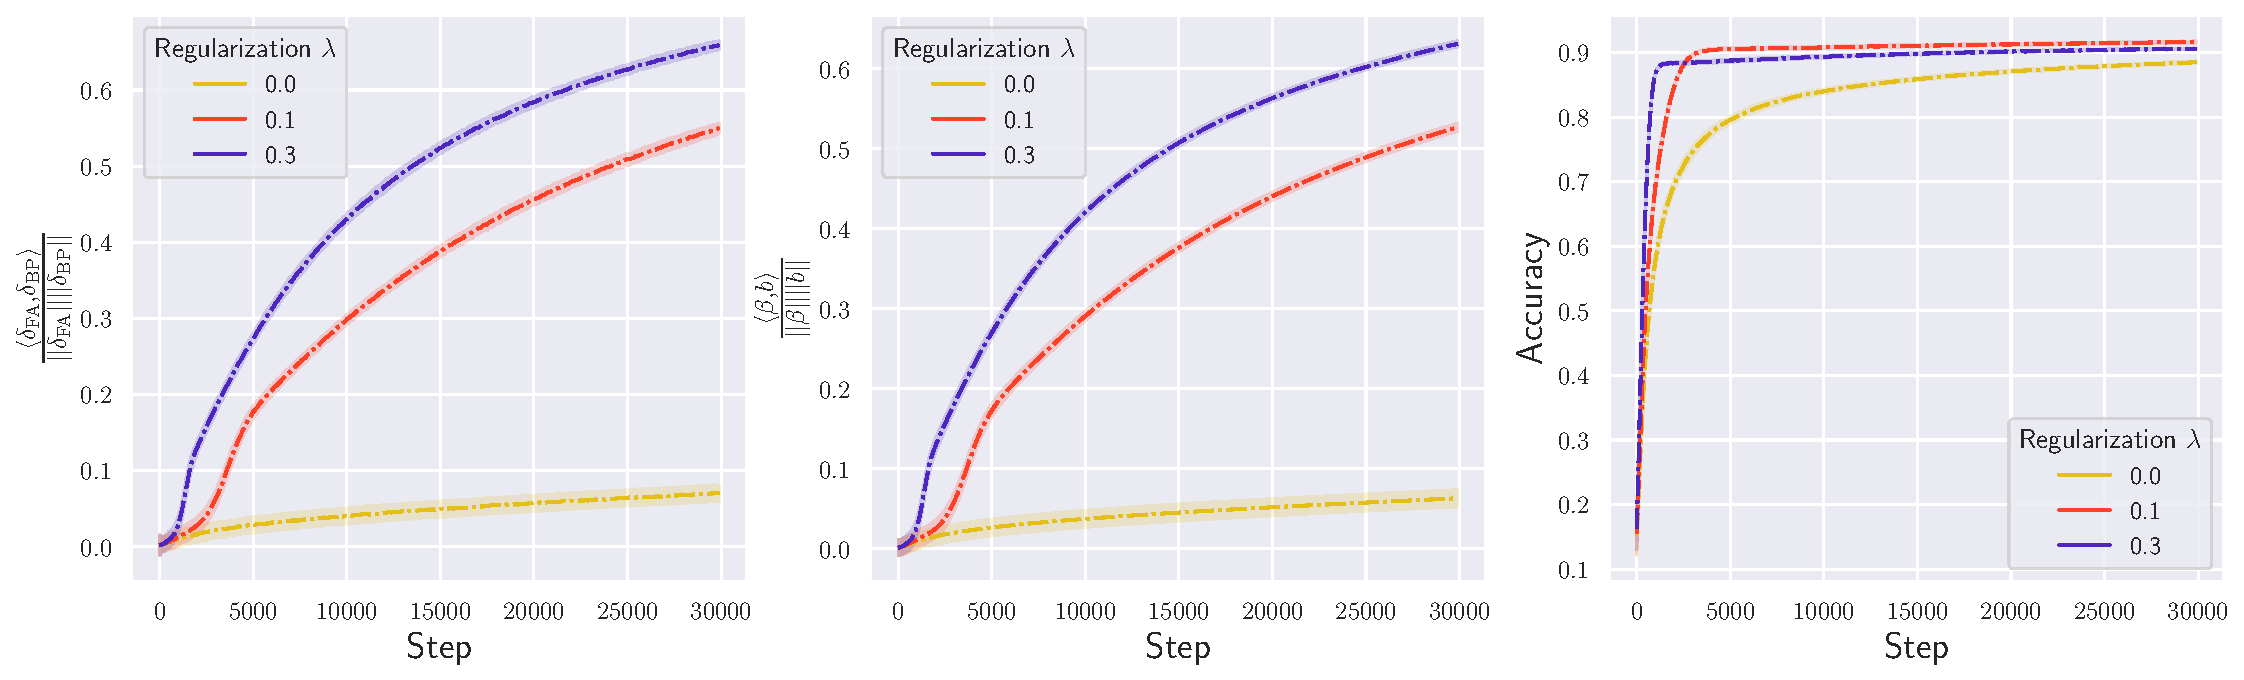
\includegraphics[width=\textwidth]{figures/mnist_2l_v6_horizontal.pdf}
  \caption{Comparisons on alignment and accuracy for feedback alignment algorithm with $\lambda=0,0.1,0.3$. The left figure shows alignment defined by $\cos \angle(\dbp(h),\dfa(h))$, and right figure shows the accuracy on the test set. The dashed lines and corresponding shaded areas represent the means and the standard deviations over $10$ runs with random initialization.}
  \label{fig:mnist}
\end{figure}
